% Setting the document's class and font size.
\documentclass[12pt,a4paper]{article}
% Importing the geometry package, allowing the tightening of margins.
\usepackage[nomarginpar,headheight=10mm,bottom=27mm]{geometry}
% Importing an important maths formatting tool
\usepackage{amsmath}
% Import all the mathematical symbols we may need, e.g. \rightarrow
\usepackage{amssymb}
% Colorise the text at will. e.g. \color{red} \color[rgb]{1.00,0.00,0.00} {HTML}{FF7F00}??
\usepackage{xcolor}
% Importing the package used to present graphics.
\usepackage{graphicx}
% Importing a package to deal with captions outside the usual. e.g. captionof
\usepackage{caption}
% Importing a package allowing the changing of caption formats
\usepackage{subcaption}
\DeclareCaptionFormat{custom}{\textbf{#1#2}\textit{\small #3}}
\captionsetup{format=custom,width=0.4\textwidth,skip=0pt}
% Setting the location of graphics used in the thesis.
\graphicspath{{Images/}}
% Importing package allowing for table creation
\usepackage{tabularx}
% Importing a package allowing for justification of text.
\usepackage{ragged2e}
% Importing the package allowing referencing
% \usepackage[backend=biber,style=alphabetic,natbib=true,url=false,doi=true]{biblatex}
\usepackage[]{biblatex}
\addbibresource{Bibliography/Bibliography.bib}
% Import the package allowing the invoking of multiple columns of text.
\usepackage{multicol}
\usepackage{lipsum}


\begin{document}
    \begin{flushleft}
        \LARGE{Bayesian Optimisation of Branching Aliphatic Polyester Thermosets}

        \vspace{0.5cm}
        \large{29\textsuperscript{th} March 2025}

        \vspace{0.25cm}
        \large{Thomas Højlund-Dodd, James Elliott}
    \end{flushleft}

    \begin{center}
        \begin{large}
            \textbf{Abstract}
        \end{large}
        \begin{justify}
            \begin{normalsize}
                Traditionally the abstract serves to inform a reader, in short, what the paper is about and what the most salient findings were.
                At present, with no work whatsoever, I can make an attempt at this.
                This paper addresses the question of whether the manufacture of bio-based branching thermoset polyesters can be optimised to improve their strengths.
                It does this by presenting a proxy for strength, means by which this is tested, means by which thermosets are manufactured and associated hyperparameters, and finally the results associated with the optimisation routines attempted.
                The most salient finding was that Bayesian optimisation successfully optimised the proxy variable in a sample efficient fashion, improving upon common deterministic techniques such as grid sampling.
                (Insert some figures to  support this claim here).
            \end{normalsize}
        \end{justify}
    \end{center}

    \begin{multicols}{2}
        \section{Introduction}
        The introduction is traditionally a section which enlightens the reader as to the background of the work.
        It can be used to reveal the breadth of the topic via the discussion of research previously undertaken on the subject areas at hand.
        This section also aims to provide a reader an understanding of the direction we as the authors have taken to address the null hypothesis presented herein.
        So we must provide an interesting question to be addressed, reasoning behind why it has been selected, what has previously been done to address the matter, and then finally what we proposed to do with our work.
        This should lead us nicely on to what we did in the method section.
        For clarity's sake it is always good to: Tell them what you are gonna tell them. Tell them. Then tell them again. The same rules apply for presentation of material.

        Global climate change has spurred a variety of political actions globally; one measure widely adopted has been adoption of more diverse supplies of energy (reducing reliance upon traditional energy vectors such as coal, oil, and gas).
        A leading form of renewable energy which has seen strong uptake globally has been wind power, which requires wind turbines; these harness aeolian kinetic energy to rotate generators and generate renewable electricity.
        Wind turbines manufactured by this industry have grown substantially since its inception.
        Towers have grown taller and blades longer.
        Criticism has been levelled at the industry because the vast majority of blades which have been manufactured using thermosetting plastic.
        These blades are made of this because of the strengths attained per mass, but the criticism is of the issue of disposal.
        The issue of disposal is simply the hatred of landfill. This is somwhat justified.
        In the context of carbon cycling this is carbon neutral;locked away carbon is returned to its original place in the ground\dots
        Work previously has been focussed on how to recycle these products to avoid the criticism levelled (quote danish scientists at aarhus who made a very clever degradable form of thermoset recently).
        This work instead takes a different view on the matter- one of long term carbon cycling.
        If thermoset material was made from bio-based resources and optimised to be as strong as traditional resources, then it could be conceivable that this would be carbon negative in a sense.
        (ITS NOT THOUGH- MAKE THIS CLEAR- CALL IT THE ENDOGENIC RETURN PRINCIPLE.)
        We will therefore focus upon the improvements we could make to a simple class of polyester thermoset called poly(glycerol itaconate citrate).
        Perhaps the thesis should feature a standalone section on the endogenic return principle and its groundings- such that it can be spoken of without people getting the impression that I am trying to be carbon negative (people get exceedingly cross if they think I am pulling a fast one on them with respect to carbon neutrality terminology.)
        The endogenic return principle is something more fundamental than simply carbon capture storage- CCS is badly defined. This could be a way around this ambiguity, but some clear definitions would have to be generated.

        \section{Method}
                This chapter will elucidate the various practicalities associated with scientifically researching the research questions posed in the introduction.

        \begin{equation}
                y=f(x_1,x_2,x_3)
            \label{eq:1}
        \end{equation}

        \begin{equation}
            f:\mathbb{R}^n \rightarrow \mathbb{R}
            \label{eq:2}
        \end{equation}

        \begin{equation}
            f(\mathbf{x}):\mathbf{x}=(x_{n},x_{n+1},x_{n+2})
            \label{eq:3}
        \end{equation}

        \begin{equation}
            \begin{split}
                &R-\textcolor[HTML]{EB7D3C}{COOH}+\textcolor[HTML]{1DB1ED}{HO}-R'\rightarrow\\
                &R-\textcolor[HTML]{EB7D3C}{CO}\textcolor[HTML]{1DB1ED}{O}-R'+\textcolor[HTML]{EB7D3C}{H}-\textcolor[HTML]{1DB1ED}{O}-\textcolor[HTML]{1DB1ED}{H}
            \end{split}
            \label{eq:4}
        \end{equation}

        \begin{equation}
            \begin{split}
            RCOOH+H&OR'\rightarrow\\
            &RCOOR'+H_{2}O
            \end{split}
            \label{eq:5}
        \end{equation}

            \subsection{Background on Chemical System Researched}
                The chemical system was a branching polyester by the name of poly(glycerol itaconate citrate).
                It is based on three simple monomers all of which are readily available bio-based feedstocks- glycerol, itaconic acid, and citric acid.
                When heated for an extended period of time these polyesterify, which is to say, undergo esterification in a chained fashion.
                Due to the multi-functional nature of these chemicals this generates branching polyesters, which can cross-link with themselves, creating a thermoset product.
                \begin{center}
                    \captionsetup{format=custom,width=0.4\textwidth,skip=0pt}
                    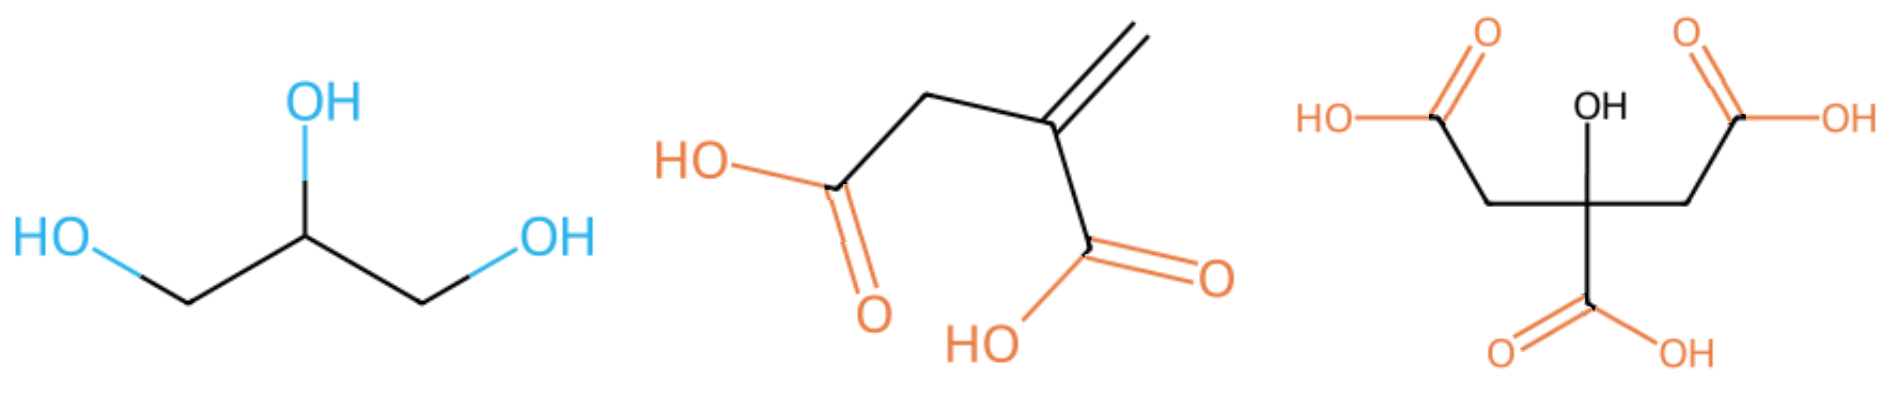
\includegraphics[width=.50\textwidth]{MonomersGroupHighlighting}
                    \captionof{figure}{\footnotesize{Skeletal diagrams of chemicals studied. Left: Glycerol. Centre: Itaconic acid. Right: Citric acid. Functional groups considered likely to be taking part in the esterification are coloured: Blue for hydroxyl groups, orange for carboxyl groups.}}
                    \label{fig:MonomersGroupHighlighting}
                \end{center}

                \begin{center}
                    \captionsetup{format=custom,width=0.4\textwidth,skip=0pt}
                    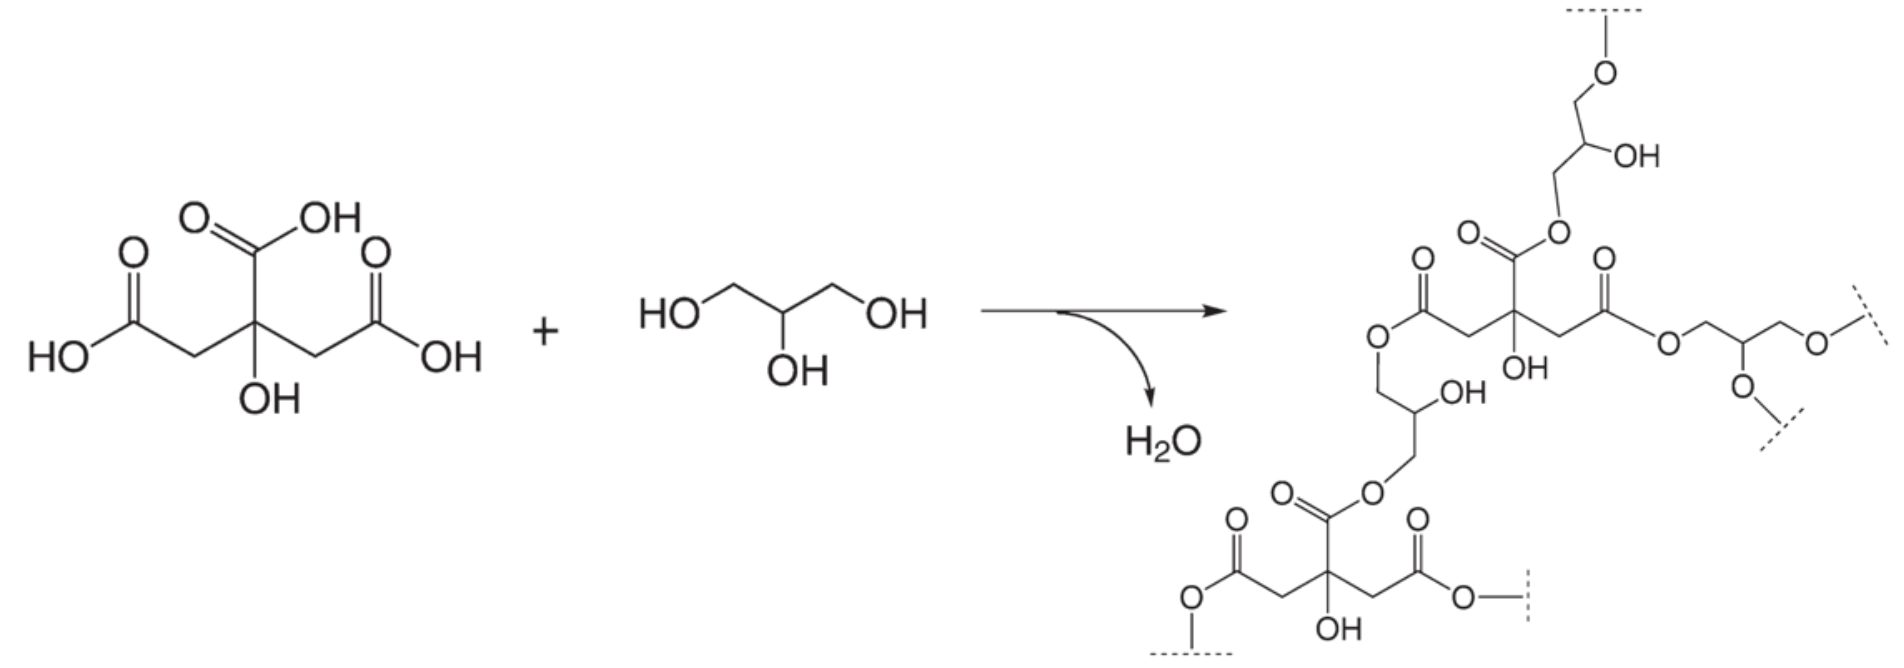
\includegraphics[width=.50\textwidth]{Polyesterification}
                    \captionof{figure}{\footnotesize{Skeletal diagram presenting the polycondensation reaction between a triol (glycerol) and a triacid (citric acid). Adapted from}}
                    \label{fig:IntroductionPolyesterification}
                \end{center}

            \subsection{Target Variable Selected and How to Measure It Practically}
                Given the proof-of-concept nature of this project we elected to use a proxy variable for strength.
                This would be mass loss; the mildly naive rationale behind this was as follows:
                For each ester link generated during the polyesterification process a water molecule is generated.
                If the heating temperature is above 100oC, which is above the boiling point of water, then water should naturally evaporate over the course of the polyesterification reaction.
                This would generate a mass loss between the start mass of the various monomers, and the end mass of the polyesterified thermoset product.
                We hence make two basic assumptions: firstly, mass loss is directly proportional to the number of ester linkages generated.
                Secondly, we assume that the number of ester linkages generated should be proportional to the number of successful cross-links within the final 3D structure of the thermoset.
                Thirdly and finally, we assume that the number of cross-links generated in the final 3D structure of the thermoset is proportional to the tensile strength exhibited by the thermoset.


                \begin{figure*}[htb]
                    \captionsetup{format=custom,width=0.8\textwidth,skip=0pt}
                    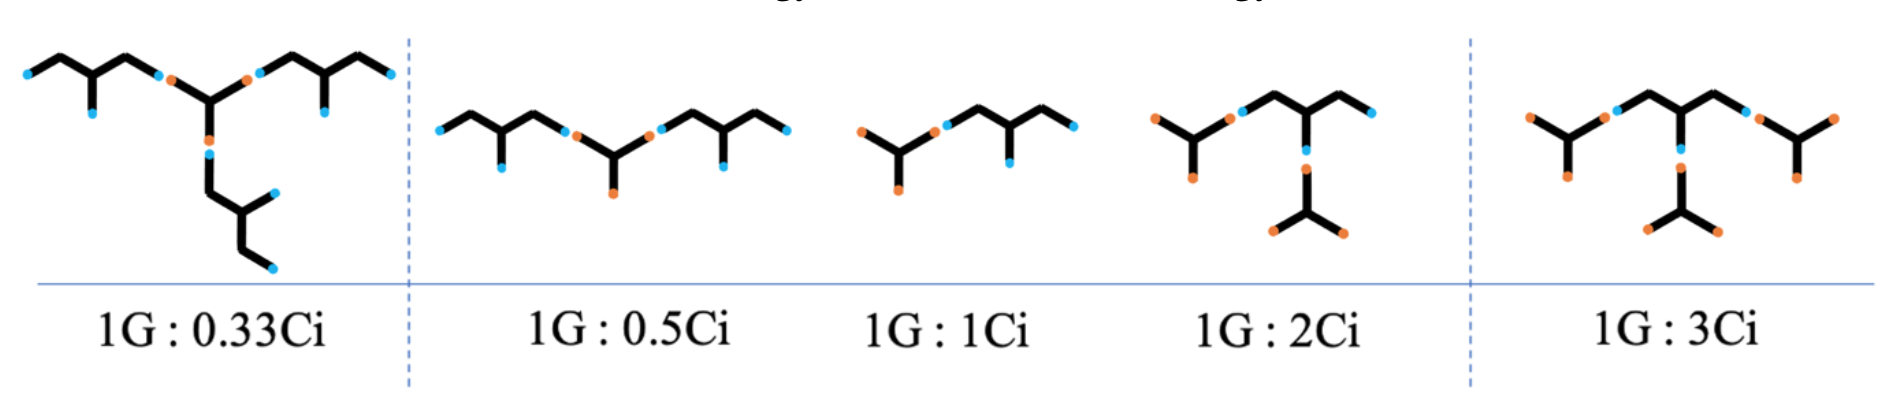
\includegraphics[width=\textwidth]{MonomerMixing}
                    \captionof{figure}{\footnotesize{Illustration of stoichiometric ratios between glycerol (G) and citric acid (Ci) and possible repeat units.}}
                    \label{fig:SecondMonomer}
                \end{figure*}

                It is therewith trivial to discover the value of this proxy variable- one simply weighs the mass of monomers used beforehand and the mass of the resultant thermoset after the polyesterification (See equation ??).
                Important is the problem of how to call an end to the polyesterification process.
                This ended up taking the form of an arbitrary gradient, beyond which the polyesterifiation would be terminated.

                \begin{figure*}[htb]
                    \captionsetup{format=custom,width=0.8\textwidth,skip=0pt}
                    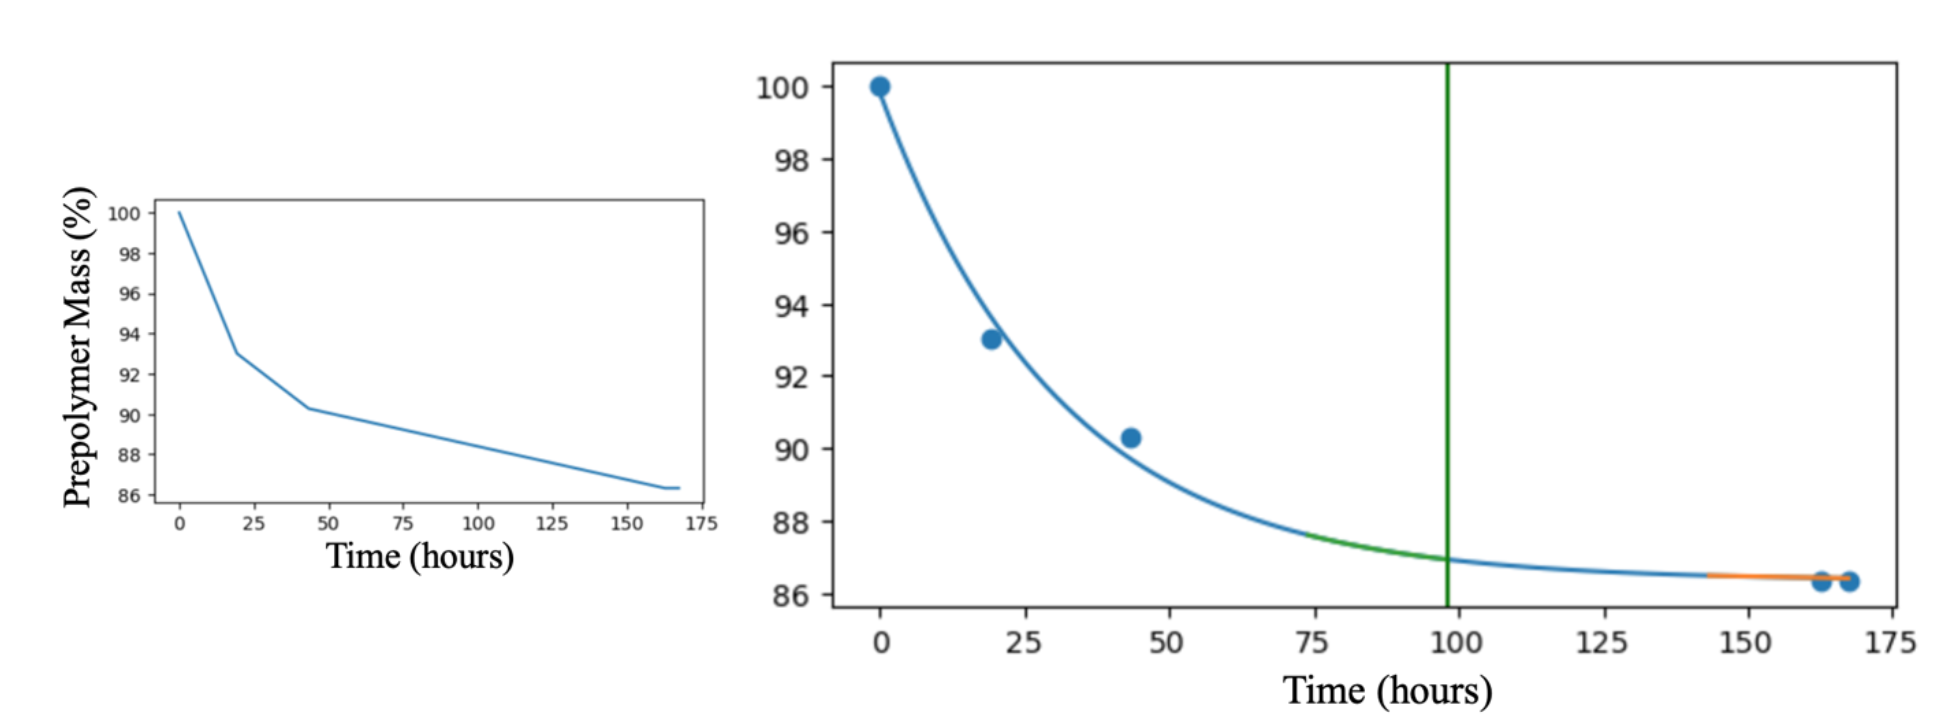
\includegraphics[width=\textwidth]{PrepoolymerMassVsTime}
                    \captionof{figure}{\footnotesize{Left: Prepolymer mass loss over time, data points connected by straight lines. Right: Prepolymer mass loss over time, data points scattered, and blue exponential curve fitted. Green vertical line shows time at which target gradient reached, and straight green tangent line exponential shows linear fit for last 24 hours of data. Orange line gives the latest 24hr tangent available at the time of graph drawing.}}
                    \label{fig:PrepoolymerMassVsTime}
                \end{figure*}

            \subsection{Predictor Variables, How to Tune Them Practically, and the Parameter Space}
                Given that poly(glycerol itaconate citrate) is comprised of three monomeric components, it becamce clear that the chemical stoichiometry would be the primary means by which properties could be tuned.
                This meant building a balancing system for the various compositions possible, and placing some bounds on the parameter space.
                (Provide the graphics used in the first year report here...)

                \begin{figure*}[htb]
                    \captionsetup{format=custom,width=0.8\textwidth,skip=0pt}
                    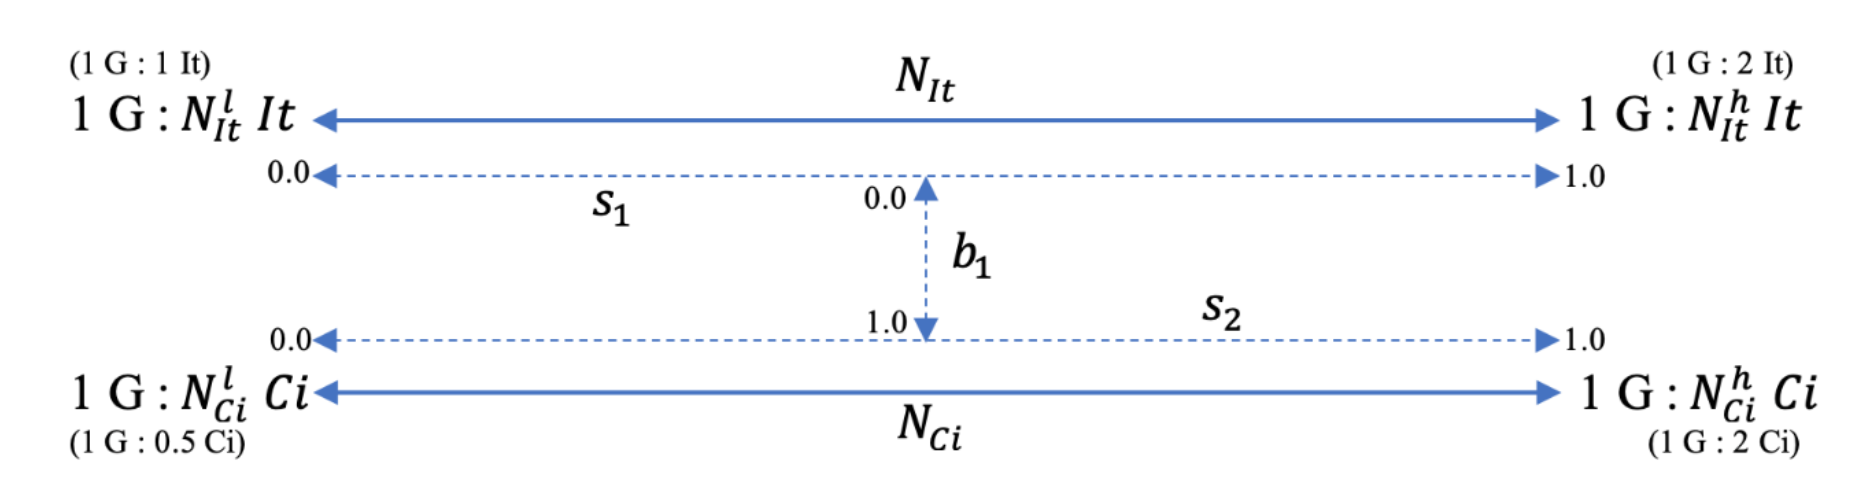
\includegraphics[width=\textwidth]{QuantificationOfMonomerMixing}
                    \captionof{figure}{\footnotesize{Visualisation of 3D optimisation parameter space for the P(GCiIt) problem.}}
                    \label{fig:QuantificationOfMonomerMixing}
                \end{figure*}

            \subsection{Bayesian Optimisation of the Variables and How it was Implemented Computationally and Practically}
                Given the target variable and predictor variables, a prior could be built over the parameter space.
                This was achieved using various forms of deterministic random sampling techniques.
                Once the prior was generated, this could be leveraged to carry out Bayesian optimisation in various forms.
                Description of the various stepping methods et cetera.
            
            \subsection{Benchmark Techniques}
                To prove the sample efficient nature of Bayesian optimisation we used a number of deterministic grid sampling techniques.
                These were grid, quasirandom, and pseudorandom, and used the entire sample limit we had presribed.
                Naturally, grid was the most representative of the parameter space, and found a good coupld of points.
                Whilst, quasirandom under performed relatively, and pseudorandom failed miserably\dots
                Some benchmarks have been developed, these are presented in figure ??.



        \section{Results}
        This results section is dedicated to presenting and contrasting the various optimisations undertaken during the research.
        It opens by presenting the space-filling deterministic sampling routines, which act as simple benchmarks for the progress of the Bayesian techniques.
        It then moves onto the various Bayesian techniques trialled.

            \subsection{Benchmark Deterministic Space-Filling Sampling}

                \begin{figure*}[htb]
                    \captionsetup{format=custom,width=0.8\textwidth,skip=0pt}
                    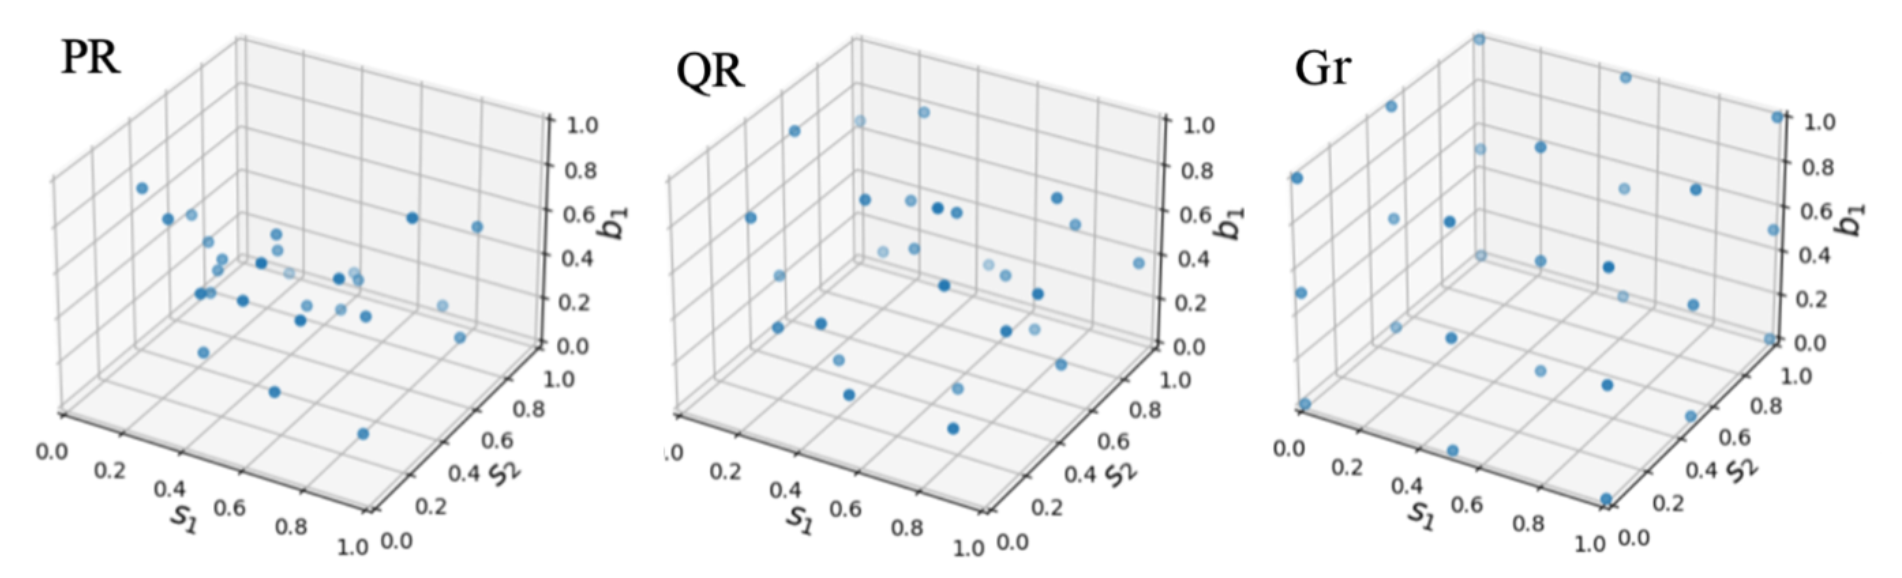
\includegraphics[width=\textwidth]{DeterministicBenchmarks}
                    \captionof{figure}{\footnotesize{Comparison of space-filling sampling techniques and distribution of 27 samples across the entire 3D parameter space of the P(GCiIt) problem. G: Grid sampling technique, QR: Quasirandom sampling technique, PR: Pseudorandom sampling technique.}}
                    \label{fig:DeterministicBenchmarks}
                \end{figure*}

                Insert table of results here.
            
            \subsection{Bayesian Techniques}
                
                \begin{figure*}[htb]
                    \captionsetup{format=custom,width=0.9\textwidth,skip=0pt}
                    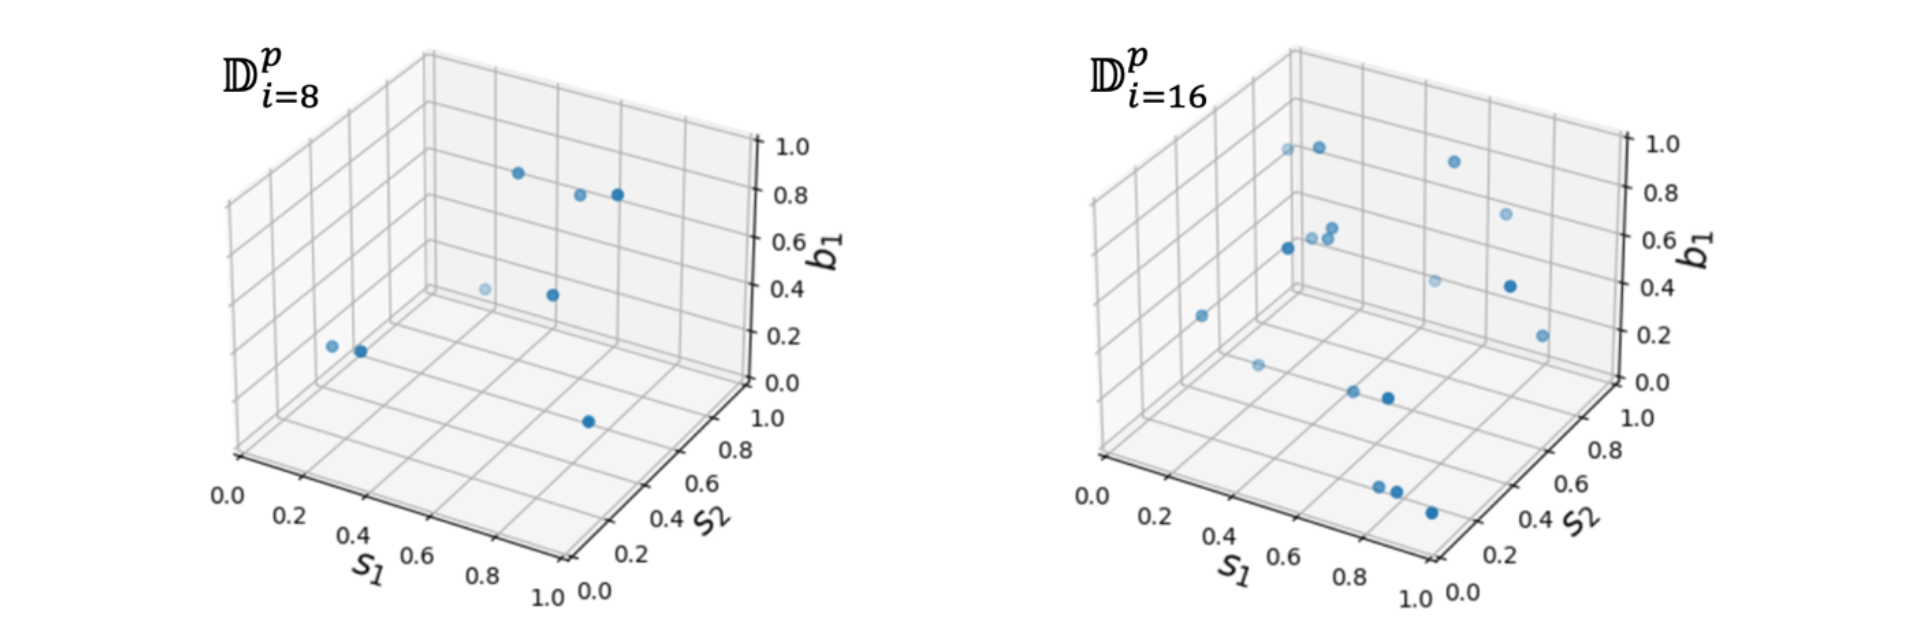
\includegraphics[width=\textwidth]{BayesianPriors}
                    \captionof{figure}{\footnotesize{Visualisation of the two representative prior datasets quasirandomly across the 3D parameter space of the P(GCiIt) system. : Eight sample prior dataset. : Sixteen sample prior dataset.}}
                    \label{fig:BayesianPriors}
                \end{figure*}

            \subsection{Comparisons of Optimisation Progressions}
                The optimisation progressions are presented to show the progress of optimisations and how they break the simple benchmarks laid out earlier.

                \begin{figure*}[htb]
                    \captionsetup{format=custom,width=0.9\textwidth,skip=0pt}
                    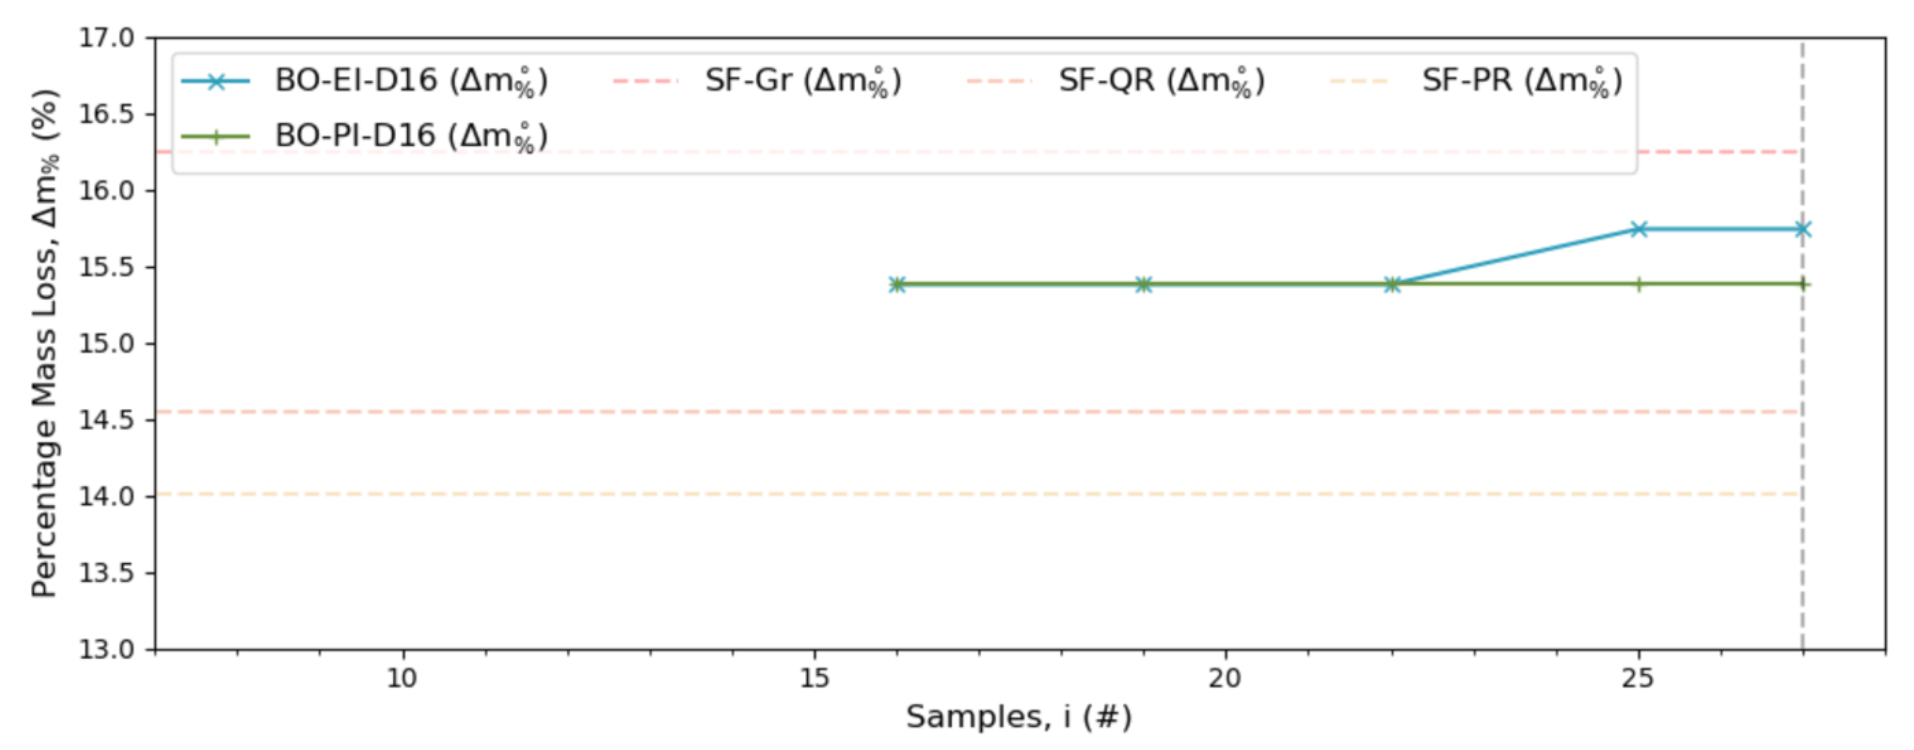
\includegraphics[width=\textwidth]{SmallPriorOptimisationProgression}
                    \captionof{figure}{\footnotesize{Graph describing optimisation progression with respect to best global optimum discovered at any given iteration for BO-EI-D16 and BO-PI-D16. Black dashed vertical line denotes ???. Crosses or pluses distributed along solid lines denote the ??? at the end of an iteration. SF-Gr/QR/PR: Space-filling Grid/Quasirandom/Pseudorandom techniques. BO: Bayesian optimisation method. PI: Probability of improvement acquisition function. EI: Expected improvement acquisition function. D16: 16-sample prior-initialising dataset.}}
                    \label{fig:SmallPriorOptimisationProgression}
                \end{figure*}
            
                \begin{figure*}[htb]
                    \captionsetup{format=custom,width=0.9\textwidth,skip=0pt}
                    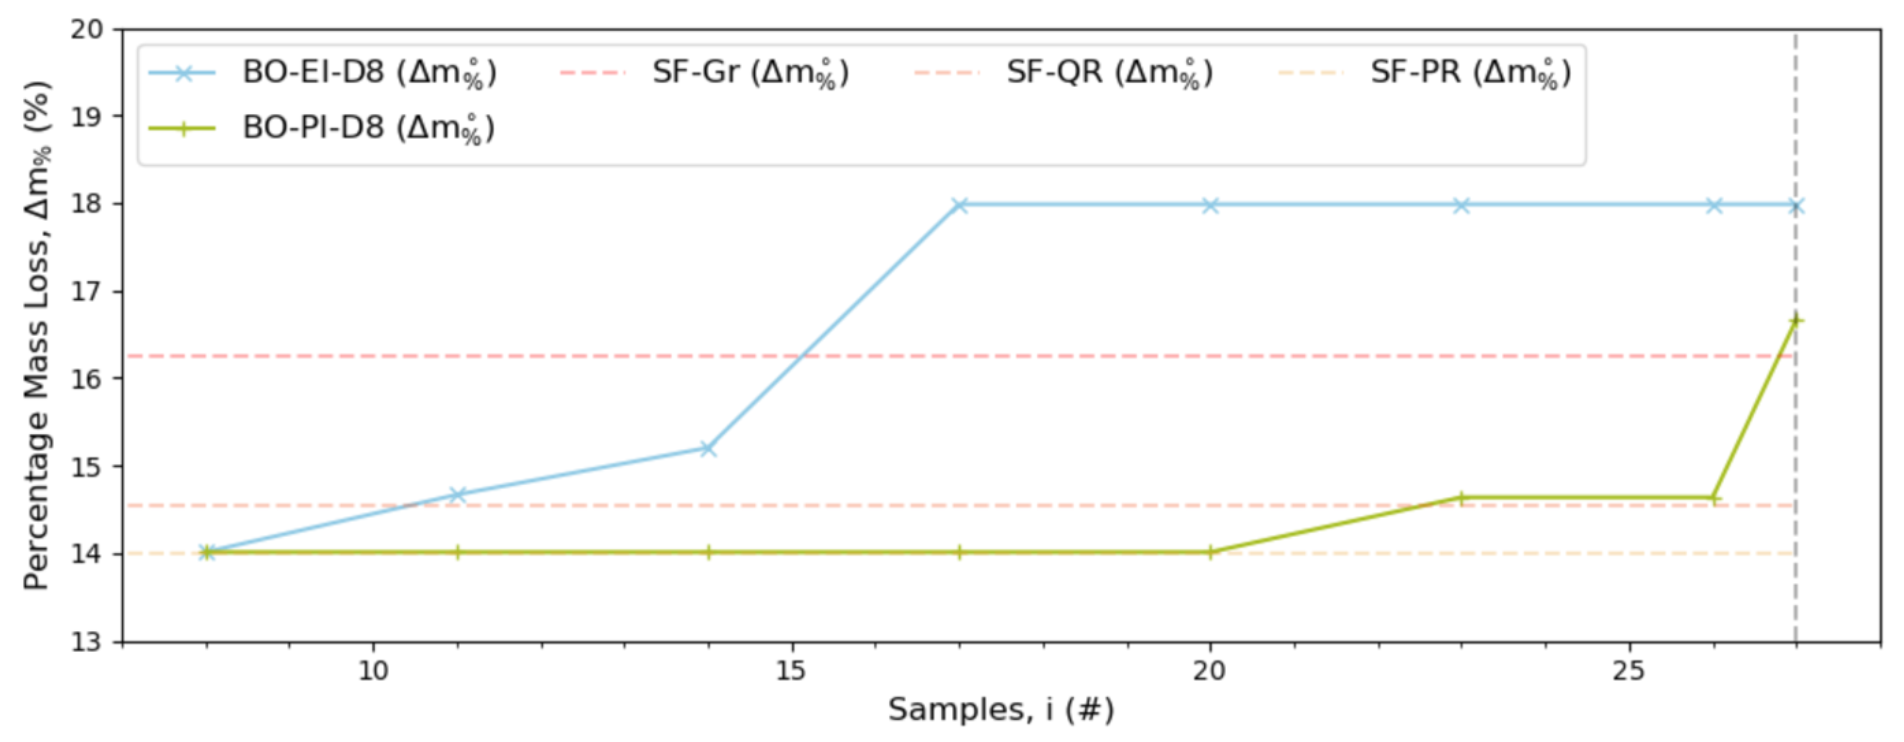
\includegraphics[width=\textwidth]{LargePriorOptimisationProgression}
                    \captionof{figure}{\footnotesize{Graph describing optimisation progression with respect to best global optimum ??? discovered at any given iteration for BO-EI-D8 and BO-PI-D8. Black dashed vertical line denotes ???. Crosses or pluses distributed along solid lines denote the ??? at the end of an iteration. SF-Gr/QR/PR: Space-filling Grid/Quasirandom/Pseudorandom techniques. BO: Bayesian optimisation method. PI: Probability of improvement acquisition function. EI: Expected improvement acquisition function. D8: 8-sample prior-initialising dataset.}}
                    \label{fig:LargePriorOptimisationProgression}
                \end{figure*}

                Insert table of results here.

        \section{Discussion}
        The discussion comprises all of the notable findings (set in context) drawn from the datasets objectively presented in the results section.
            \textbf{Prior-Forming Dataset Size Effect}
            ahbx

            \textbf{Acquisition Function Effect}
            ahbx

            \textbf{Bayesian Optimisation Sample Efficiency}
            ahbx

            \textbf{Stochastic Sampling Problem}
            ahbx

            \textbf{Global Optimum Estimation}
            ahbx

            \textbf{Optimum Stoichiometry Derivation}
            ahbx

        \section{Conclusion}

        \lipsum[2-4]

    \end{multicols}{2}

\end{document}